\hypertarget{a-kozossegi-let-szabalyai}{%
\section{A közösségi lét szabályai}\label{a-kozossegi-let-szabalyai}}

A Budapest School egy közösségi iskola: a gyerekek együtt tanulnak és
alkotnak, a tanárok csapatokban dolgoznak, és a szülők is egy elfogadó
közösség részének érezhetik magukat. A tagok --- a tanárok, a gyerekek,
a szülők és az adminisztrátorok --- azért csatlakoznak a közösséghez,
mert itt szeretnének lenni, és itt érzik magukat boldognak,
egészségesnek és hasznosnak. A közösség azért fogad be új tagokat, hogy
nagyobb, erősebb közösség lehessen.

\hypertarget{partnerseg}{%
\paragraph{Partnerség}\label{partnerseg}}

A tanulásszervezők és a családok közös célja, hogy közösségük a gyerekek
fejlődését együtt támogassa. A tanulás holisztikus szemlélete révén a
gyerekeknek egyszerre kell jó kapcsolatot ápolniuk saját társaikkal,
partnerségben lenniük tanáraikkal, és meghallaniuk a szülők feléjük irányuló
kéréseit. A tanulás célját a gyerekek maguk határozzák meg, azok az
értékek, rituálék viszont, melyek a mindennapjaikat meghatározzák,
túlmutatnak az egyénen, és a közösség céljait szolgálják oly módon, hogy
az az egyes családok életvitelével is összhangban legyen.

Minden tanulóközösségnek feladata ezért, hogy az együttműködésük, a
közösségi szabályaik, a házirendjük meghatározásakor a családok
véleményét, javaslatait is kikérjék, és úgy hozzanak döntést, hogy az
mindenki számára kellően biztonságos és elég jó döntés legyen.

Ez vonatkozhat a mindennapi eszközök használatára, a közlekedésre, az
együtt, tanulással eltöltött egyéni és csoportos idő arányaira, a
közösen megtartott ünnepekre, jeles napokra, mindazokra a kérdésekre,
melyek közösségi döntések, és hatással lehetnek az egyén fejlődésére.

\hypertarget{alapcsoportok}{%
\paragraph{Alapcsoportok}\label{alapcsoportok}}

A Budapest School iskola kisebb
tanulóközösségekből áll (\ref{a-budapest-school-tanulokozossegei}.~fejezet, \pageref{a-budapest-school-tanulokozossegei}.~oldal). Ez a gyerekek és tanárok elsődleges közössége:
a gyerekek számára ez az a közösség, akikkel együtt járnak iskolába, együtt
alakítják az iskolájukat, a tanárok számára ez az a csapat, akikkel együtt
dolgoznak, hogy létrehozzák, fenntartsák és fejlesszék a tanulóközösség
gyerekeinek tanulási környezetét.

A tanulás egysége a
modul (\ref{tanulasi-tanitasi-egysegek-a-modulok}.~fejezet, \pageref{tanulasi-tanitasi-egysegek-a-modulok}.~oldal).
Egy modul csoportjában a közös érdeklődésű és célú gyerekek tanulnak
együtt, mert együtt boldogabban, hatékonyabban el tudják érni a
céljukat.

\hypertarget{sajat-szabalyok}{%
\paragraph{Saját szabályok}\label{sajat-szabalyok}}

A tanulóközösség és akár egy-egy modul kereteit, szabályait a résztvevők
alakítják ki. Pontosabban a tanárok~felelőssége és feladata, hogy minden
tanár és gyerek számára elfogadható, betartható, releváns és értelmes
szabályok legyenek. (Mikroiskola esetén a tanulásszervező tanárok,
modulok esetén a szaktanárok és a tanulásszervező tanárok közösen.)

Mind a gyerekek, mind a tanárok javasolhatnak új szabályokat vagy
szabályváltoztatást. Minden egyes gyereknek és tanárnak hozzájárulását
kell adnia minden javaslathoz, mondván: \emph{,,it's good enough for
now and safe enough to try''}, azaz: „elég jónak és biztonságosnak
tartom, hogy kipróbáljuk''.

Ebből következik, hogy minden tanulóközösségnek saját házirendje,
szabályai lehetnek, és modulonként alakulhat, hogy mit, mikor, hogyan és
kivel csinálnak a résztvevők.

A szabályok alakításának elsődleges szándéka mindig az legyen, hogy a
gyerekek fejlődése, tanulása, alkotása és a közösség működése egyre jobb
legyen.

\begin{figure}
\centering
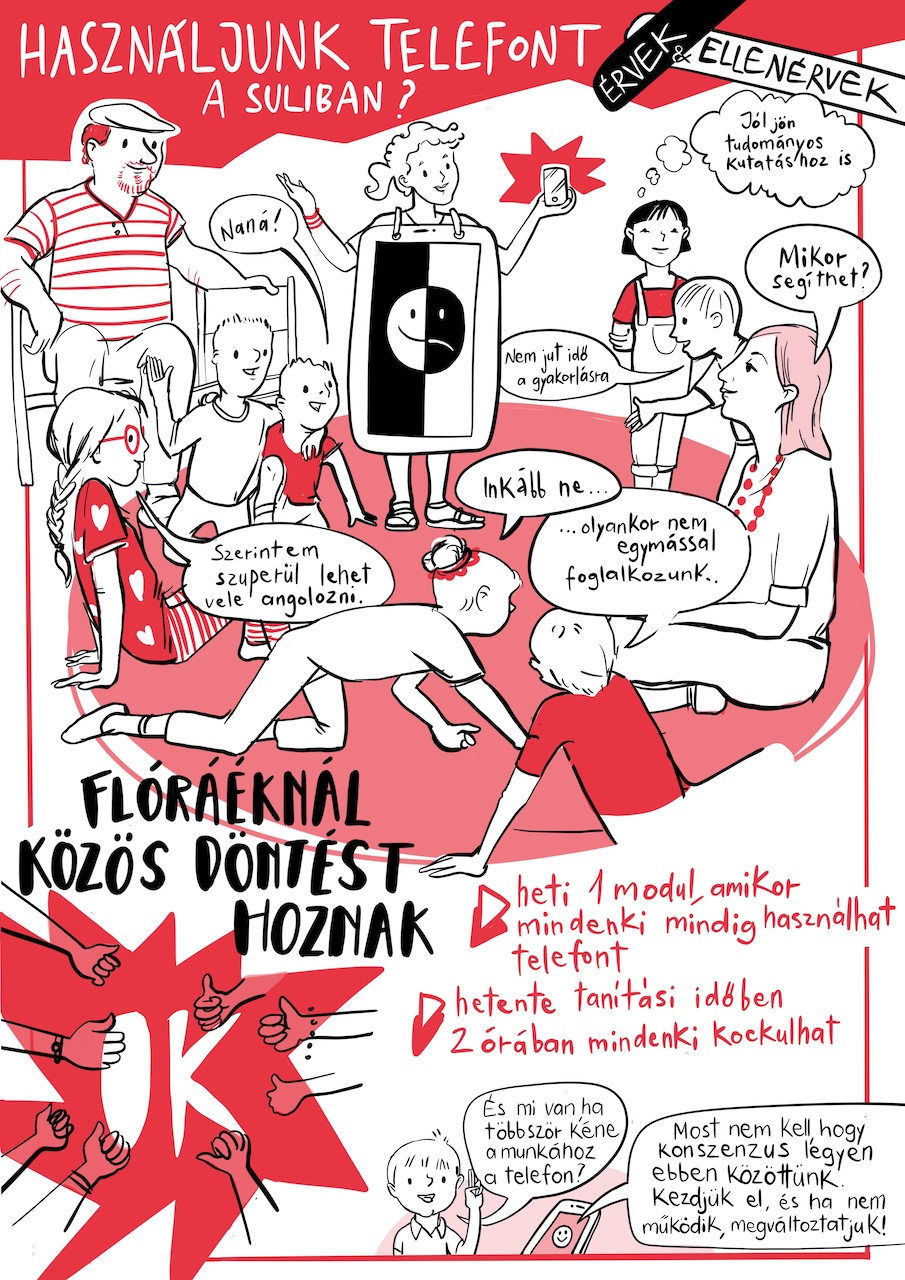
\includegraphics{pics/5b_dontes.jpg}
\caption{A tanulóközösség egy családias közösség.}
\end{figure}

\hypertarget{konfliktusok-feszultsegek-kezelese}{%
\subsection{Konfliktusok, feszültségek
kezelése}\label{konfliktusok-feszultsegek-kezelese}}

Tudjuk, hogy a Budapest School szereplői, a gyerekek, a tanárok, a
szülők, a pedagógiai program, a kerettanterv, a fenntartó, a szomszédok,
az állami hivatalok között feszültségek és konfliktusok alakulhatnak ki,
mert különbözőek vagyunk, különbözőek az igényeink. A feszültségekre és
a konfliktusokra a Budapest School olyan lehetőségként tekint, amelynek
együttműködésen alapuló megoldása építi a kapcsolatot, és segíti a
fejlődést.

Minden vágy, ötlet, szándék, cél, viselkedés közötti különbség, ha az
valamelyik félben negatív érzéseket kelt, feszültséget és konfliktust
okozhat. Ebbe beletartozik az is, ha valaki nem azt és úgy csinálja,
ahogy nekünk erre szükségünk van, vagy ha bármilyen okból nem érezzük
magunkat biztonságban, vagy más univerzális emberi szükségletünk
{\autocite{Rosenberg2003}} nem elégül ki.

Konfliktus alakulhat ki a gyerekek, szülők és tanárok között bármilyen
relációban, és adódhatnak egyéb, belső konfliktusok, nehézségek is akár
a család, akár a Budapest School életében, amelyek kihathatnak a
közösségi kapcsolatainkra.

\begin{figure}
\centering
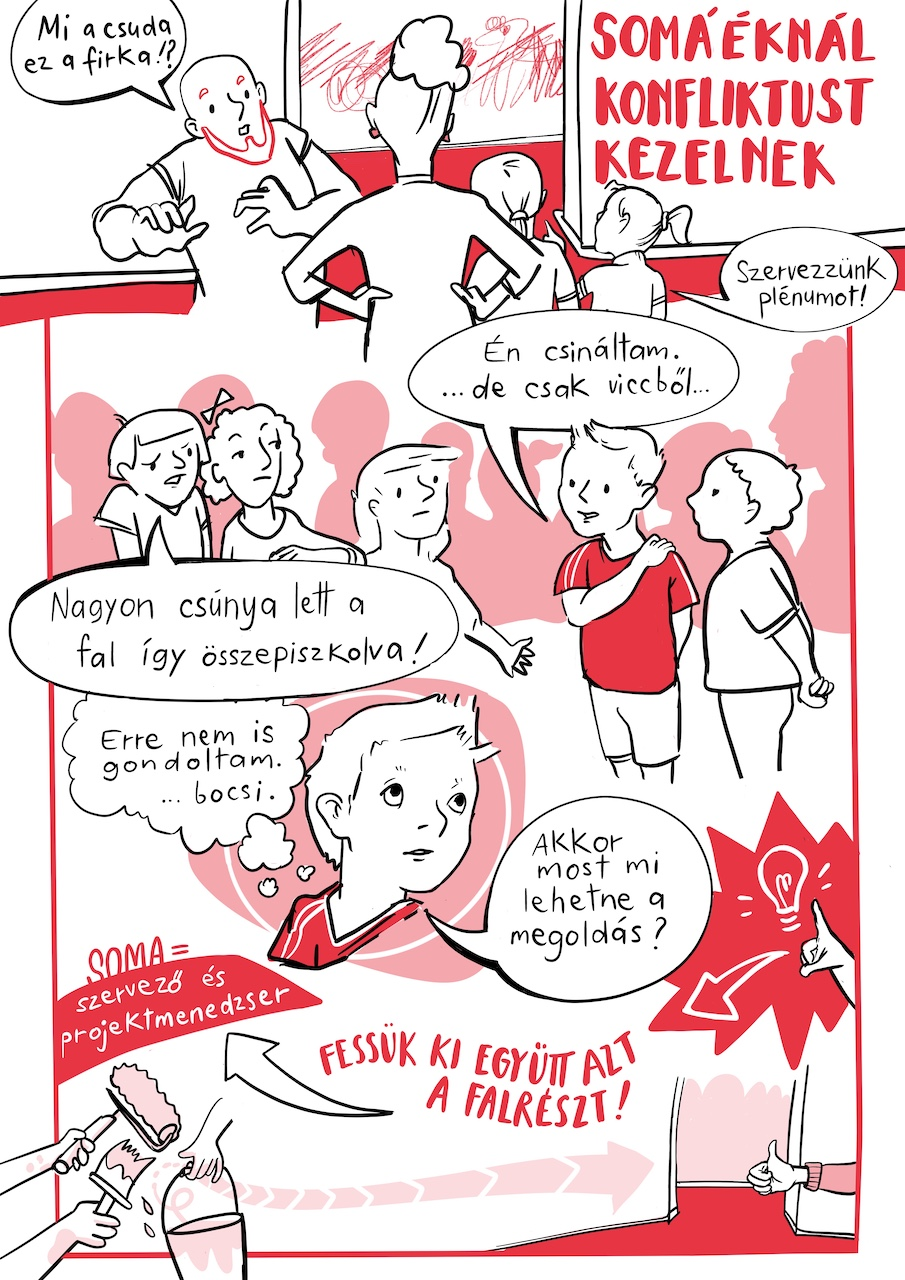
\includegraphics{pics/5a_konfliktus.jpg}
\caption{A tanulóközösség egy családias közösség.}
\end{figure}

\hypertarget{a-bps-konfliktusok-feloldasa}{%
\subsubsection{A konfliktusok feloldása a BPS-ben}\label{a-bps-konfliktusok-feloldasa}}

Az iskola partnerségen alapuló szervezetében nem autoritások, főnökök,
hivatalok, bírók oldják meg a konfliktusokat, hanem egyenrangú társak.
Az iskola feltételezi, hogy a felek tudnak gondolkodni, következtetni,
felelősséget vállalni a döntéseikért és cselekedeteikért. A kisgyerekeket
mentoraik és szüleik képviselik.

\hypertarget{alapertekek}{%
\paragraph{Alapértékek}\label{alapertekek}}

Ahhoz, hogy tényleg partneri kapcsolatban, egyenrangú\break
felekként lehessen
konfliktusokat, problémákat megoldani, érdemes közös értékeket
elfogadni.

\begin{itemize}
\item
  Először a saját változásunkon dolgozunk, mert másokat nem nagyon tudunk
  megváltoztatni, csak a magunk változásáért lehetünk felelősek.
\item
  Felelősséget vállalunk gondolatainkért, hiedelmeinkért, szavainkért
  és viselkedésünkért.
\item
  Nem pletykálunk, szóbeszédet nem terjesztünk.
\item
  Nem beszélünk ki embereket a hátuk mögött.
\item
  A félreértéseket tisztázzuk, a konfliktusokat felszínre hozzuk.
\item
  A problémákat személyesen, szemtől szembe beszéljük meg, másokat nem
  húzunk bele a problémába.
\item
  Nem hibáztatunk másokat a problémákért. Amikor mégis, akkor az
  jó alkalom arról gondolkozni, hogy miként vagyunk mi is része a
  problémának, és miként kell a megoldás részévé válnunk.
\item
  Az erősségekre több figyelmet fordítunk, mint a gyengeségekre, és a
  lehetőségekről, a megoldásokról többet beszélünk, mint a problémákról.
\end{itemize}

\hypertarget{feszultseg-felszinre-hozasa}{%
\paragraph{A feszültségek felszínre
hozása}\label{feszultseg-felszinre-hozasa}}

Olyan módszereket, folyamatokat, szabályokat, szokásokat kell
kialakítani minden közösségben, hogy legyen tere és ideje a
feszültségeket előhozni.

\begin{itemize}
\item
  Az iskolai csoportok rendszeresen egy bejelentkező
  körrel kezdik a napjukat, ahol van lehetőség a problémákat is
  megbeszélni.
\item
  A csoportok rendszeresen tartanak retrospektív gyűlést, ahol
  értékelik, mi volt jó, és mi nem volt annyira jó egy vizsgált időszakban.
\item
  Évente legalább kétszer a tanárok egymásnak, a szülők a tanároknak,
  a gyerekek a tanároknak, a tanárok a gyerekeknek szervezett formában
  visszajelzést adnak.
\item
  A gyerekek a mentorukkal rendszeresen találkoznak, és ilyenkor teret kapnak
  a felmerülő feszültségek.
\end{itemize}

\hypertarget{megbeszeles}{%
\paragraph{Megbeszélés}\label{megbeszeles}}

A Budapest School közösségének valamennyi tagja (a tanárok, gyerekek,
szülők, adminisztrátorok, iskolát képviselő fenntartó)\break
vállalja:

\begin{itemize}
\item
  A közösség mindennapjaival kapcsolatos konfliktusok esetén elsőként az
  abban érintett személynek jelez közvetlenül.
\item
  A személyes kritikát mindig privát csatornán fogalmazza meg először,
  ha kell, akkor segítő bevonásával.
\item
  Bármelyik fél jelzése esetén lehetőséget biztosít arra, hogy a vitás
  kérdést közvetlenül megbeszéljék, a folyamatban részt vesz.
\item
  Szakítás, kilépés, lezárás előtt legalább három alkalommal megpróbál
  egyeztetni.
\item
  Az egyeztetésre elegendő időt hagy, amely legalább 30 nap,
 vagy\break
 (ha ennél több időre van szükség) a másik féllel megállapodott
  idő.
\item
  Teljes figyelemmel, nyitottsággal, a probléma megoldására fó\-ku\-szál\-va
  igyekszik feloldani a konfliktust, és közösen megoldást találni a
  problémára.
\end{itemize}

Összefoglalva: ha problémánk van egymással, akkor azt megbeszéljük. Nem
okozunk egymásnak meglepetést, mert vállaljuk, hogy rögtön elmondjuk
egymásnak gondjainkat.

\hypertarget{kozvetito-bevonasa}{%
\paragraph{Közvetítő bevonása}\label{kozvetito-bevonasa}}

Ha úgy érezzük, hogy a személyes egyeztetés nem vezetett megoldásra, a
tárgyalást külső segítség bevonásával folytatjuk. Ez lehet egy másik
csoporttag, egy tanár, vagy egy teljesen külsős mediátor.

Amikor bármely fél közvetítőt kér, akkor a másik ezt elfogadja. Nem
mondhatjuk azt, hogy ~\emph{„de hát mi magunk is meg tudjuk oldani a
konfliktust''}.

\hypertarget{eszkalalas}{%
\paragraph{Eszkalálódás}\label{eszkalalas}}

Ha két fél nem tudja megoldani a konfliktust, akkor kérhetnek segítséget
a \texttt{segitseg@budapestschool.org} címen, amire 48 órán belül kell
választ kell kapniuk. Az e-mail kezeléséért az iskola fenntartója felel.

\hypertarget{megallapodasok}{%
\paragraph{Megállapodások}\label{megallapodasok}}

Ha az egyeztetés, tárgyalás és közvetítő bevonása során sikerül
valamilyen megoldást vagy a megoldáshoz vezető folyamatot egyeztetni, a
felek \emph{megállapodnak} abban, hogy ki mit tesz, vagy milyen
szabályokat alakítanak ki, illetve hogy mennyi időt adnak egymásnak,
hogy kipróbálják, sikerült-e feloldani a konfliktust. Segíteni szokott a
kérdés, hogy \emph{most megállapodtunk vagy csak beszéltünk róla?}

Nagyobb konfliktusok esetén jó gyakorlat, és ezt bármely fél kérheti, hogy
írásban is rögzítik a megállapodást. Ez lehet egy papírfecni is vagy
egy e-mail. Lényege nem a formátum, hanem hogy minden fél emlékezzen a
megállapodásra.

\hypertarget{ha-az-egyeztetes-sikertelen}{%
\paragraph{Ha az egyeztetés
sikertelen}\label{ha-az-egyeztetes-sikertelen}}

Ha a felek között az egyeztetés sikertelen volt, vagy a megoldási
javaslat nem működött, a feleknek ezt írásban meg kell állapítaniuk.
Erre azért van szükség, hogy egyetértés legyen közöttük abban, hogy
értik, a másik fél sikertelennek érzi az egyeztetést.

\hypertarget{lezaras}{%
\paragraph{Lezárás}\label{lezaras}}

Az egyeztetés sikertelensége esetén elengedjük egymást. De ez a végső
megoldás.

\hypertarget{kiemelt-konfliktusok}{%
\subsection{Kiemelt konfliktusok}\label{kiemelt-konfliktusok}}

\hypertarget{gyerek-gyerek-konfliktus}{%
\subsubsection{Gyerek---gyerek
konfliktus}\label{gyerek-gyerek-konfliktus}}

A mindennapokban a gyerekek akarva-akaratlanul is belecsöppennek\break
olyan
helyzetekbe, amikor a közösségben vagy interperszonális kapcsolataik
során megborul a mindennapi egyensúly. Ezekben a konfliktushelyzetekben
leginkább a felborult egyensúly helyreállítására törekszünk
\emph{helyreállító konfliktusfeloldási technikával}.

A helyreállító konfliktusfeloldás alaptézise az, hogy minden ilyen
megborult egyensúlyi állapot egy lehetőség valaminek a megújítására,
újragondolására. A résztvevők egy külső személy segítségével (általában
a jelen lévő tanáréval) alakítják a megoldást, egészen addig, amíg az
eredmény mindenki számára a konfliktus feloldását, azaz a
megborult egyensúly helyreállítását jelenti.

A folyamat során a konfliktusban részt vevő összes személy elmondja az
érzéseit, meglátását a felmerülő helyzettel kapcsolatban, valamint az
én-közléseken túl a szükségleteikről is beszélnek. Ezen szükségletek
képezik a megoldás alapját, azaz ezeket egy tető alá hozva feloldhatjuk
a fennálló konfliktust. Ilyenkor mindig először azokat a pontokat
keressük meg, amelyekben egyetértenek a résztvevők, hiszen ez közös
alapot szolgáltat arra, hogy a valódi feloldást megtalálhassuk.

Fontos, hogy a beszélgetésben az összes fél hallassa a hangját, és meg
is legyen hallgatva. Az értő figyelem kompetenciája is fejlődik ezen
módszer alkalmazása során, például, ha az érintett felek elmondják, hogy
mit hallottak meg abból, amit a másik elmondott.

Előfordulhat, hogy ez a folyamat nem egyből a konfliktus után indul el:
ha a résztvevők beleegyeznek, akkor a beszélgetés elhalasztható, de
lehetőleg még aznap történjen meg.

\hypertarget{gyerek-iskola-tanar-szulo-konfliktus}{%
\subsubsection{Gyerek---iskola és tanár---szülő
konfliktus}\label{gyerek-iskola-tanar-szulo-konfliktus}}

Minden gyereknek van egy mentora. A szülők számára a mentor az
elsődleges kapocs az iskolával. Ezért, ha a szülőben jelenik meg egy
feszültség, akkor elsődlegesen a mentornak jelez. Ugyanígy a mentor
közvetíti a család felé a gyerekkel kapcsolatos feszültségeket.

Ha egy gyerek vagy szülő úgy érzi, hogy egy gyereknek nem jó az iskolai
élménye, például nem tanul eleget, vagy kiközösítik, vagy csak nem
szeret bemenni, akkor feladata, hogy rögtön beszéljen a mentorral.

Ha nem sikerül a mentorral megbeszélni a konfliktust és megoldást
találni, akkor a szülőnek is lehetősége van segítőt behívni, aki lehet
egy másik tanár, másik szülő, az iskolaigazgató vagy bárki, akinek
képességeiben bízik.

Előfordulhat, hogy a tanárok vagy az iskola úgy érzik, hogy egy
gyereknek nem tesz jót a Budapest School közössége, vagy a hozzáállása
súlyosan zavarja vagy sérti a Budapest School közösséget vagy azok
tagjait. Az is lehet, hogy a tanárok vagy a Budapest School a szülővel
való kapcsolatot érzik konfliktus vagy feszültség forrásának. Ilyen
esetben ugyanígy le kell folytatni a konfliktuskezelés folyamatát, és
meg kell próbálni feloldani a feszültséget. Ennek sikertelensége esetén az
iskola írásban jelzi a családnak, hogy el fognak válni.

\hypertarget{bps-modell-egyedi-program-hazirend-be-nem-tartasaval-kapcsolatos-konfliktusok}{%
\subsubsection{BPS modell, egyedi program, házirend be nem tartásával
kapcsolatos
konfliktusok}\label{bps-modell-egyedi-program-hazirend-be-nem-tartasaval-kapcsolatos-konfliktusok}}

Amikor egy tanár, egy gyerek vagy egy tanulóközösség nem tartja be az
egyedi programot, a házirendet, vagy egyéb közösen megalkotott
szabályokat, akkor konfliktus alakul ki közte és az iskola között.
Ilyenkor szintén a konfliktuskezelés folyamatát kell alkalmazni.
